\documentclass[11pt]{article}
\usepackage[margin=1in]{geometry}
\usepackage{booktabs}
\usepackage{graphicx}
\usepackage{microtype}
\usepackage[hidelinks]{hyperref}

\title{\vspace{-2em}\textbf{Paper-list quality under a low cap}}
\author{arxivkg · generation · landmark selection}
\date{}

\begin{document}
\maketitle
\vspace{-2em}

\section*{What we did}
The committed retrieval takes a hard PPR top-40. Does relevance-filtering that list beat it, and does
the cap need to grow? Four arms over one shared pool (same adjacency-list + extracted digest; only the
landmark \emph{set} differs), disentangling \textbf{filter-type} from \textbf{count}: \texttt{fixed40}
(PPR top-40), \texttt{gate40} (0.35 cosine ancestor gate, top-40), \texttt{llm40} (drop role=unrelated
over PPR-100, capped 40 --- same count), \texttt{llm\_dyn} (same filter, soft cap 60). Scored on the
Exp-1-validated metric: direct list metrics (count, recall[gold], precision[role judge], lineage-span)
primary + the compose-judge on its trusted axes (grounding, coverage) + pairwise vs \texttt{fixed40}
(lineage asterisked); judges date-injected.

\section*{Results (8 topics, gold-3 for recall)}
\begin{center}\begin{tabular}{lrrrrrr}
\toprule
arm & count & recall & precision & coverage & overall & pair \\
\midrule
fixed40 & 40.0 & 0.742 & 0.838 & 4.125 & 4.688 & 0.0 \\
gate40 & 40.0 & 0.808 & 0.881 & 4.375 & 4.75 & 0.62 \\
llm40 & 40.0 & 0.808 & 1.0 & 4.5 & 4.75 & 0.62 \\
llm-dyn & 60.0 & 0.808 & 1.0 & 4.25 & 4.75 & 0.62 \\
\bottomrule
\end{tabular}
\end{center}
\begin{center}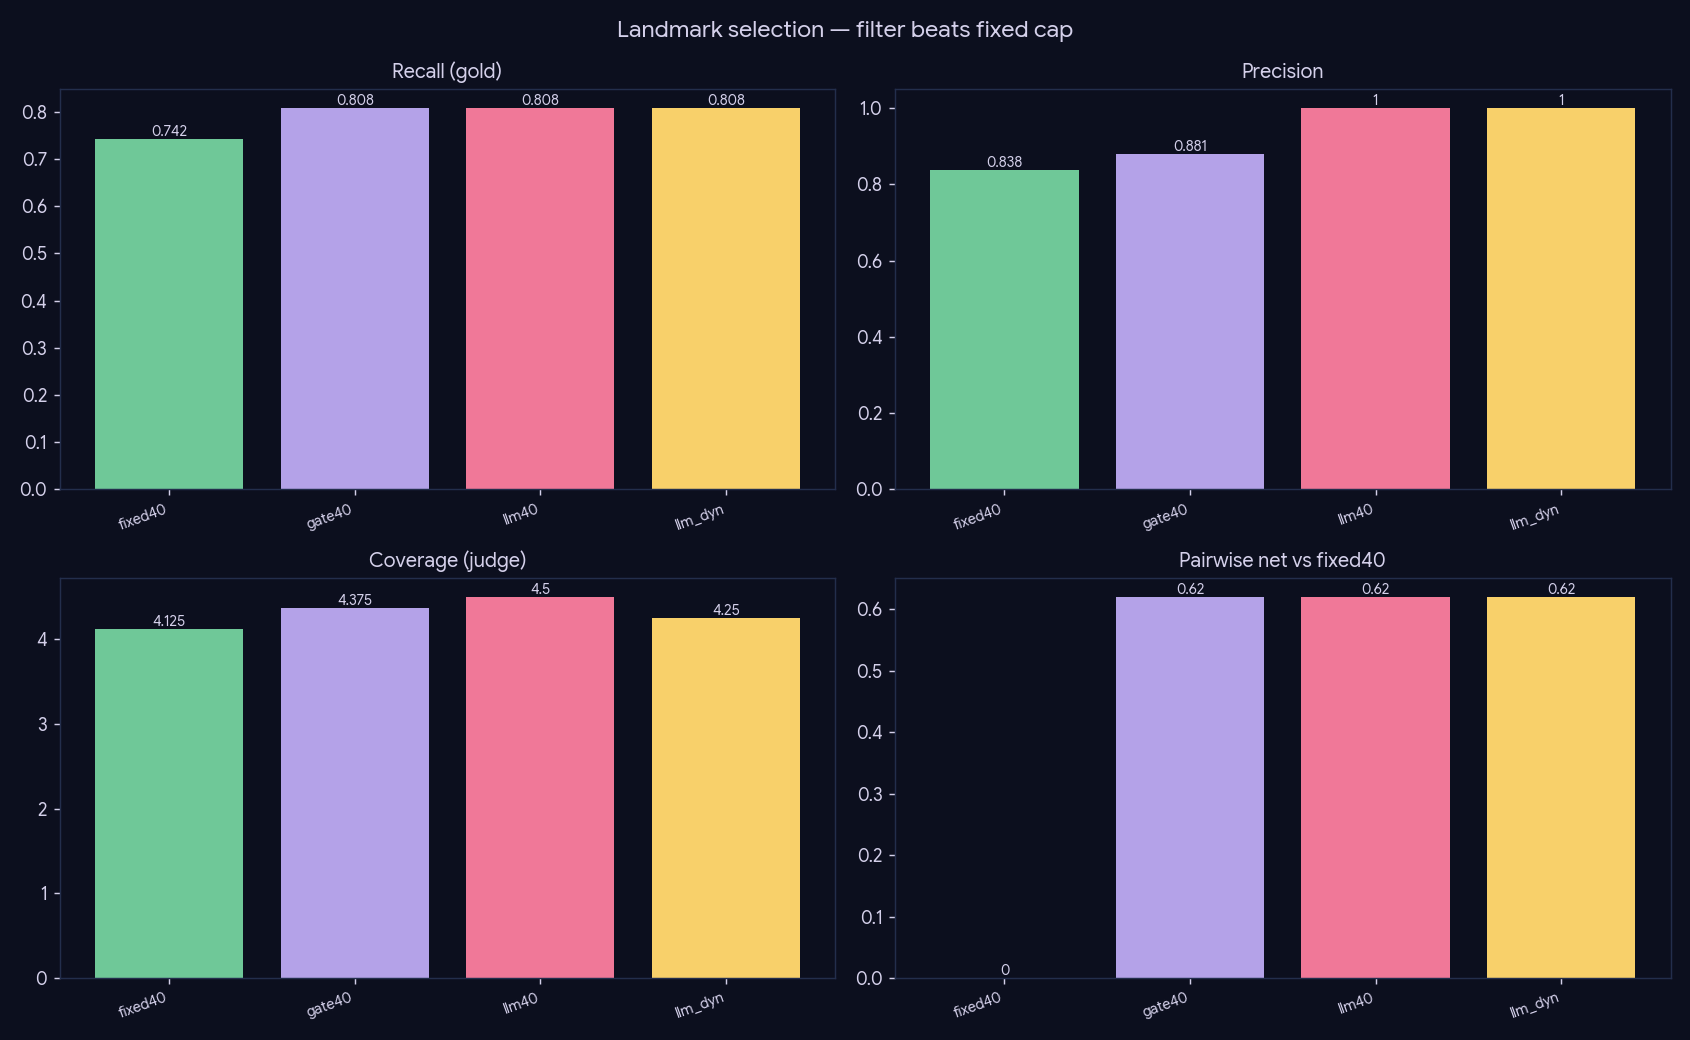
\includegraphics[width=0.95\textwidth]{../results/ablation.png}\end{center}

\section*{Conclusion}
\textbf{The win is the FILTER, not the count --- keep the list at 40 and filter for relevance; do not
expand it.} All three alternatives beat \texttt{fixed40} (recall 0.742$\rightarrow$0.808, pairwise
+0.62 = 5W/3T/0L). \textbf{\texttt{llm40} (filter at the same 40) captures the full win} --- perfect
precision (1.0), full recall (0.808), best coverage (4.5) --- at zero size increase. \textbf{\texttt{llm\_dyn}
(60) does not beat \texttt{llm40} (40)} (identical recall/precision/pairwise, slightly lower coverage:
cleaner beats bigger). The cheap \texttt{gate40} gets $\sim$80\% of the win; the LLM filter adds the
precision polish (0.881$\rightarrow$1.0). So replace the hard top-40 with a relevance-filtered top-40 ---
the cheap gate at minimum, the LLM filter for precision-max. Caveat: n=8; the robust signal is the
direct metrics, pairwise margins are modest and on validated axes only.

\end{document}
